\subsection{ Quality Evaluation Across Aggregate Functions }
In these experiments we evaluate quality of the recommended visualizations produced by proposed techniques 
 across different aggregate functions namely: \emph{Count, Sum, Average, Min, and Max}. 
The dataset used is $Flight$ database for flight delays in year 2008 obtained from 
The U.S. Department of Transportation's Bureau of Transportation Statistics (BTS) with 
size 250 K tuples \footnote { http://www.transtats.bts.gov/}. 
The dataset contains 10 dimension attributes and 10 measures attributes. 
We run this experiment to assess the quality of the recommended views 
over each aggregate function \emph{separately} 
 with a space size(SP)=$1 \times 10 \times 10=100$ possible views and 
the deviation metric is Earth Movers Distance (EMD). All Experiments were executed 
5 times and obtained the averaged results, we concerned with evaluating the 
the accuracy and utility of views produced by the proposed algorithms along 
limited number of views (referred as Views Limit) $R$ and various sets of top deviated views $K$. In experiments, the analyst
posed a query\\
 $Q:$ select * from ontime2008 where uniquecarrier ='American Airlines Inc.' \\ 
We implement two baseline strategies SeeDB baseline strategy processes the entire data 
and does not discard any views ($SeeDB baseline$). It thus provides an upper bound on 
latency and accuracy and lower bound on error distance.
The other baseline strategy we evaluate is the random strategy ($SeeDB_Rnd$) that 
returns a random set of k aggregate views as the result. This strategy gives a lower bound on 
accuracy and upper bound on error distance: for any technique to be useful, it must do 
significantly better than $SeeDB_Rnd$.

In the next experiments, we vary $R$ — the number of limited visualizations that explored denoted as \emph{Views Limit} 
to recommend $K=20$ visualizations and measure the accuracy, and error-distance for each of our
strategies along different aggregate functions.\\

In summary, $Sela$ and $DimsHisto$ algorithms both produce results with accuracy $>80\%$ and near-zero utility
distance for all aggregate functions and a variety of $R$ Views Limits particularly when Views Limits=60 views as shown in figures \ref{fig:SumA2},\ref{fig:AvgA2}, and \ref{fig:CountA2}. Moreover, they produce results with $100\%$ accuracy and zero distance error after that limit. $Sela$ does slightly better than $DimsHisto$ as $Sela$ evaluates the recommended views by capturing the change of the selectivity ratios of dimension attributes that create views in both result set and reference set however, $DimsHisto$ scores accuracy $100\%$ in figure \ref{fig:CountA2} for aggregate function \emph{Count} because the generated histograms from this algorithm are similar to the views created by counting dimension attribute values across different measure attributes. Algorithm $Diff_DVal$ is the lowest accuracy and the highest distance error among other algorithms specially for aggregate functions \emph{Max and Min} as shown in figures \ref{fig:MaxA2} and \ref{fig:MinA2} as it assess recommended views based on the difference of the distinct values only. 

\begin{figure}[h]
  \begin{subfigure}[b]{0.32\textwidth}
    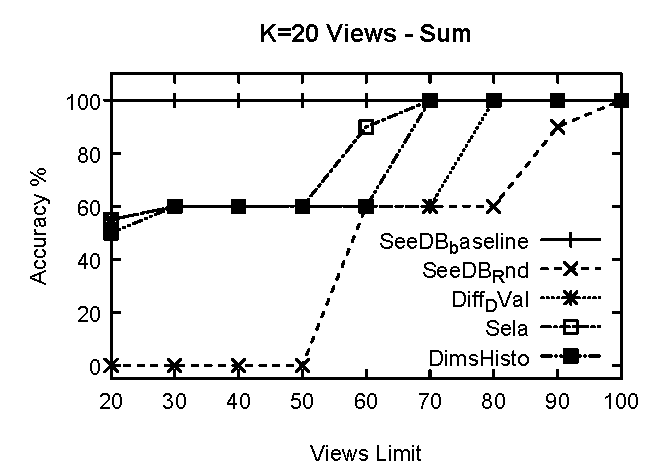
\includegraphics[width=\textwidth]{SumA2.pdf}
    \caption{Sum}
     \label{fig:SumA2}%
  \end{subfigure}
  %
  \begin{subfigure}[b]{0.32\textwidth}
    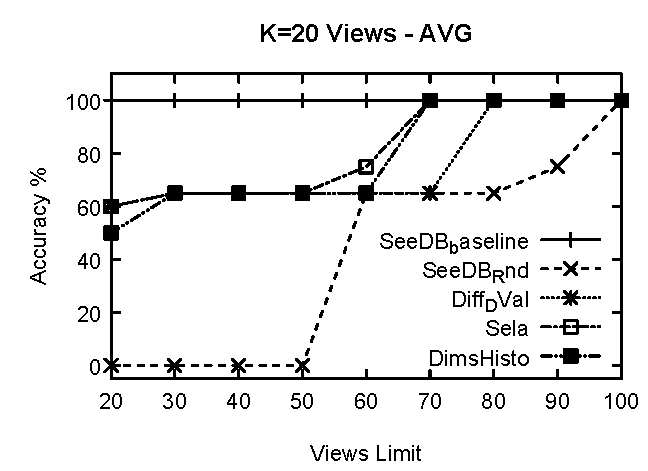
\includegraphics[width=\textwidth]{AvgA2.pdf}
     \caption{Average}
        \label{fig:AvgA2}
  \end{subfigure}
  \begin{subfigure}[b]{0.32\textwidth}
    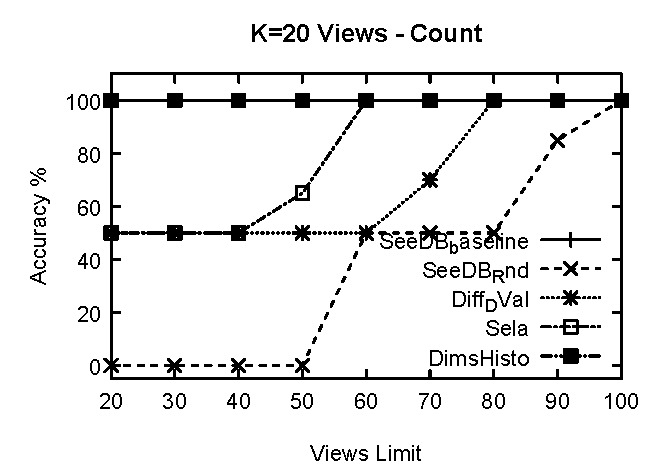
\includegraphics[width=\textwidth]{CountA2.pdf}
     \caption{count}
        \label{fig:CountA2}
  \end{subfigure}
  \caption{Accuracy on varying view space sizes for the Algorithms $Sela$ ,$Diff_DVal$, $DimsHisto$, and $SeeDB_Rnd$}
\end{figure}

\begin{figure}[h]
  \begin{subfigure}[b]{0.32\textwidth}
    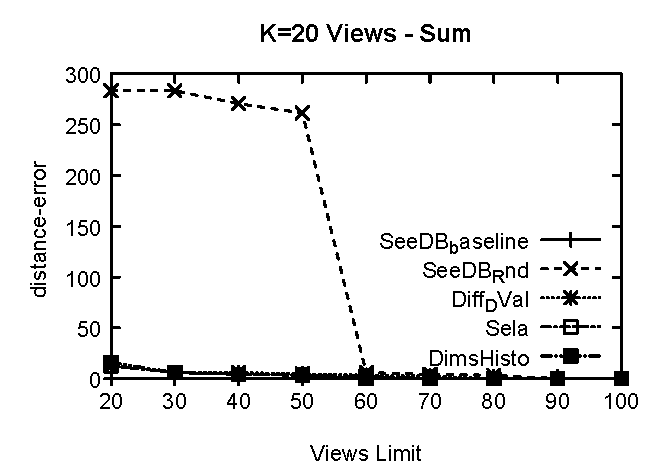
\includegraphics[width=\textwidth]{SumD2.pdf}
    \caption{Sum}
        \label{fig:SumD2}%
  \end{subfigure}
  %
  \begin{subfigure}[b]{0.32\textwidth}
    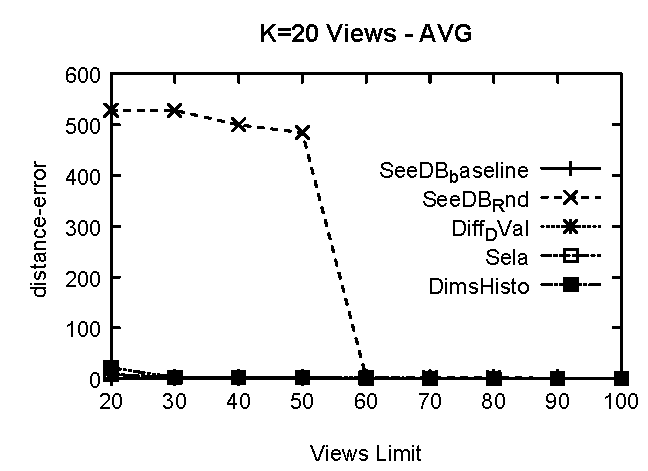
\includegraphics[width=\textwidth]{AvgD2.pdf}
     \caption{Average}
        \label{fig:AvgD2}
  \end{subfigure}
  \begin{subfigure}[b]{0.32\textwidth}
    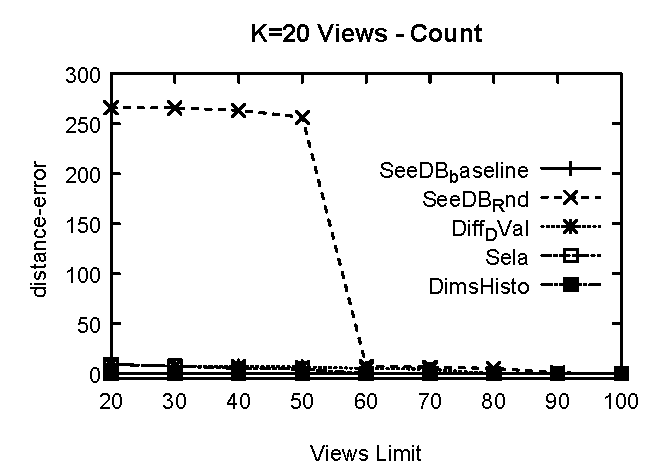
\includegraphics[width=\textwidth]{CountD2.pdf}
     \caption{count}
        \label{fig:CountD2}
  \end{subfigure}
  \caption{Distance-error on varying view space sizes for the Algorithms $Sela$ ,$Diff_DVal$, $DimsHisto$, and $SeeDB_Rnd$}
\end{figure}

As shown in figures \ref{fig:SumD2},\ref{fig:AvgD2},\ref{fig:CountD2} The proposed algorithms produce results near-zero distance-error for all aggregate functions compared with lower baseline strategy $SeeDB_Rnd$ which produce views with low quality however, the quality of the recommended views produced by the proposed algorithms is almost near to the same utilities of views output by the top baseline $SeeDB baseline$. The distance-error of results in the first view limits=20 and 30 views as shown in figures \ref{fig:MaxD2},\ref{fig:MinD2} is high specially for the aggregate function \emph{Min} because functions such as Min and Max are not docile for sampling but the proposed algorithms still score very low distance-error as shown in the figures.
 
 %\begin{center}
  \begin{figure}[h]
  \centering
  \begin{subfigure}[b]{0.42\textwidth}
    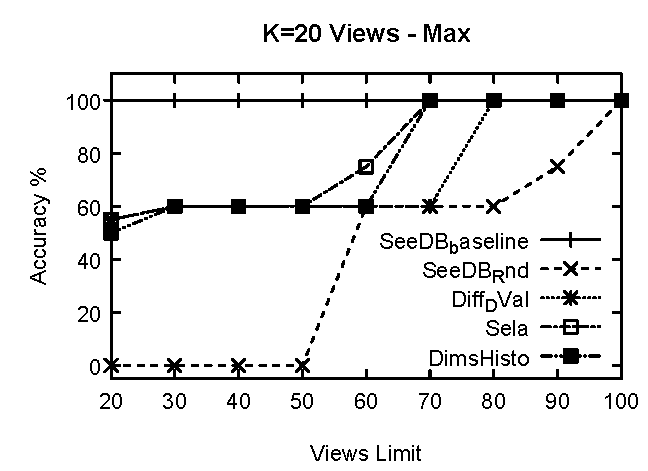
\includegraphics[width=\textwidth]{MaxA2.pdf}
    \caption{Max}
        \label{fig:MaxA2}%
  \end{subfigure}
  %
  \begin{subfigure}[b]{0.42\textwidth}
    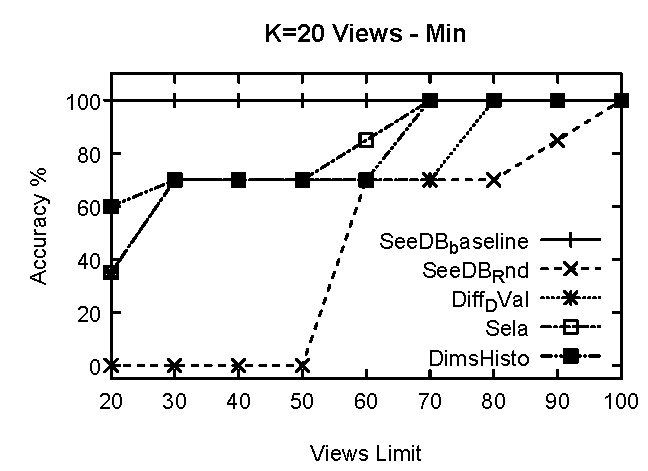
\includegraphics[width=\textwidth]{MinA2.pdf}
     \caption{Min}
        \label{fig:MinA2}
	% \caption{Accuracy on varying view space sizes for the Algorithms $Sela$ ,$Diff_DVal$, $DimsHisto$, and $SeeDB_Rnd$}
  \end{subfigure}
  \caption{Accuracy on varying view space sizes for the Algorithms $Sela$ ,$Diff_DVal$, $DimsHisto$, and $SeeDB_Rnd$}
\end{figure}
%\end{center}

%\begin{center}
  
\begin{figure}[h]
  \centering

  \begin{subfigure}[b]{0.42\textwidth}
    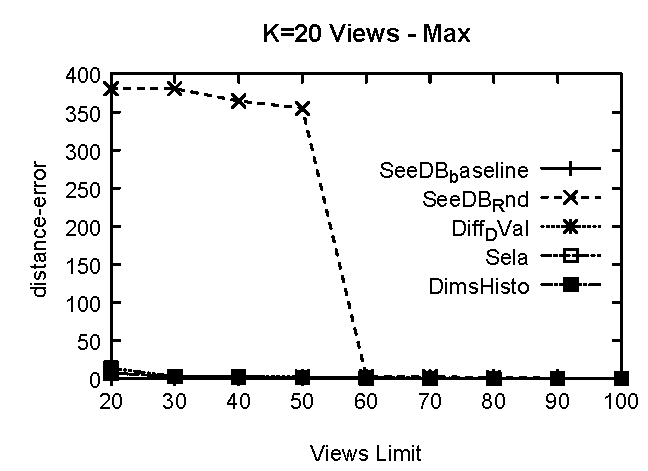
\includegraphics[width=\textwidth]{MaxD2.pdf}
    \caption{Max}
        \label{fig:MaxD2}%
  \end{subfigure}
  %
  \begin{subfigure}[b]{0.42\textwidth}
    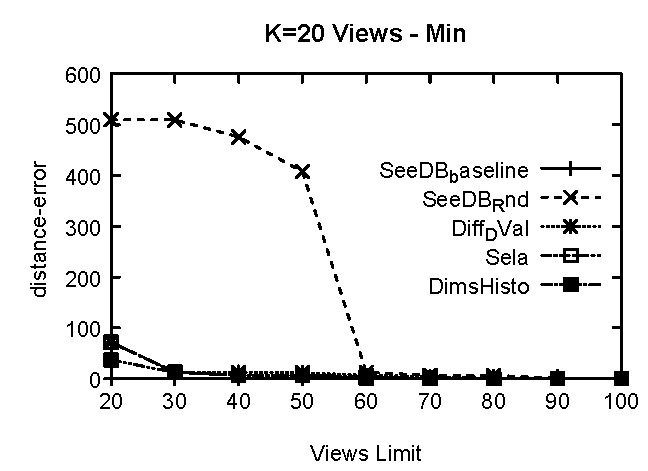
\includegraphics[width=\textwidth]{MinD2.pdf}
     \caption{Min}
        \label{fig:MinD2}
  \end{subfigure}
  
  \caption{Distance-error on varying view space sizes for the Algorithms $Sela$ ,$Diff_DVal$, $DimsHisto$, and $SeeDB_Rnd$}
\end{figure}

%\end{center}

In conclusion, the proposed techniques recommend high quality views in different views limits furthermore, the accuracy is increasing and it doesn't fluctuate along various views limits and similarly the distance-error is declining while increasing the number of explored views (views limit). In the worst cases, the accuracy and the distance-error remain fixed while increasing the number of explored views but they don't decrease. \\
%%%%%%%% Second Expr
\par In the following experiments, we vary $K$ — the number of visualizations
to recommend and fix the number of explored visualizations as \emph{Views Limit=70} and measure the accuracy, and error-distance for each of our
strategies along different aggregate functions. We pay special attention to k = 10 and 20 because empirically these k values are used most commonly.

In summary, $Sela$ and $DimsHisto$ algorithms both produce results with accuracy $100\%$ and zero distance-error when K=10 and 20 views for all aggregate functions as shown in figures \ref{fig:SumA1}, \ref{fig:AvgA1}, \ref{fig:CountA1}, \ref{fig:MaxA1}, and\ref{fig:MinA1} also algorithm $Diff_DVal$ scored accuracy $100\%$ in the first number of recommended views K=10 views. Although, $Diff_DVal$ obtains the same accuracy as $SeeDB_Rnd$ for all aggregate functions but the $Diff_DVal$ scores much better distance-error than $SeeDB_Rnd$ as shown in figures \ref{fig:SumD1}, \ref{fig:AvgD1}, \ref{fig:CountD1}, \ref{fig:MaxD1}, and\ref{fig:MinD1}. As discussed in the previous experiment, the $DimsHisto$ scores accuracy $100\%$ specifically when the aggregate functions \emph{Count} it is also succeeded to recommend views with $100\%$ and zero distance-error for aggregate functions \emph{Sum, Average, and Count} as shown in figures \ref{fig:SumA1}, \ref{fig:AvgA1}, and \ref{fig:CountA1}. In addition, we find that $Sela$ and $DimsHisto$ algorithms produce high quality views with $100\%$ accuracy and zero distance-error for \emph{Max} aggregate function , also they obtain $>75\%$ and $<0.2$ distance error for \emph{Min} aggregate function when k=70 (Views Limit ) as shown in \ref{fig:MaxD1} and \ref{fig:MinD1} receptively.

\begin{figure}[h]
  \begin{subfigure}[b]{0.32\textwidth}
    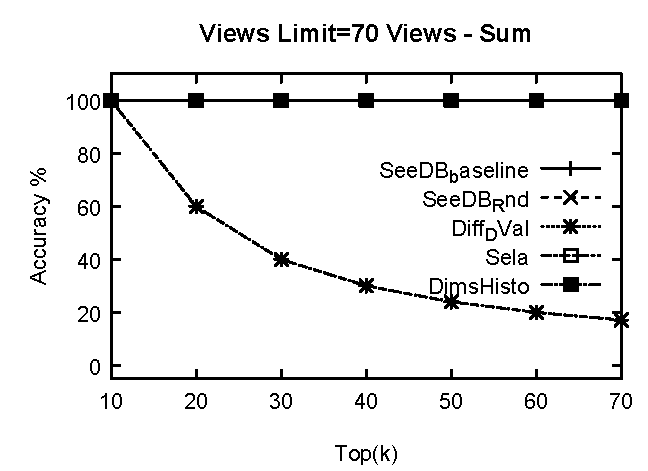
\includegraphics[width=\textwidth]{SumA1.pdf}
    \caption{Sum   }
        \label{fig:SumA1}%
  \end{subfigure}
  %
  \begin{subfigure}[b]{0.32\textwidth}
    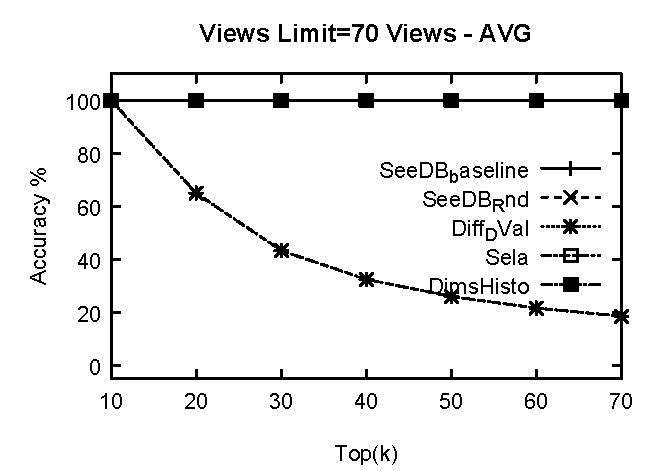
\includegraphics[width=\textwidth]{AvgA1.pdf}
     \caption{Average  }
        \label{fig:AvgA1}
  \end{subfigure}
  \begin{subfigure}[b]{0.32\textwidth}
    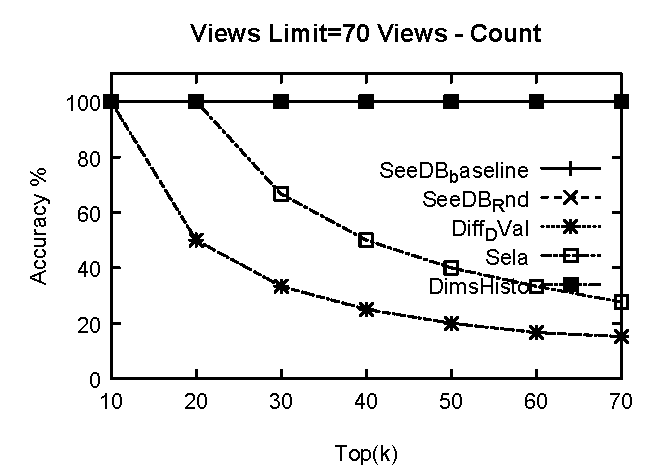
\includegraphics[width=\textwidth]{CountA1.pdf}
     \caption{count  }
        \label{fig:CountA1}
  \end{subfigure}
  \caption{Accuracy on varying view space sizes for the Algorithms $Sela$ ,$Diff_DVal$, $DimsHisto$, and $SeeDB_Rnd$}
\end{figure}

The following figures describe the distance error for the proposed algorithms, we find that although $Diff_DVal$ approach score the same accuracy produced by $SeeDB_Rnd$ strategy but it obtains very low distance error along all aggregate function compared with $SeeDB_Rnd$ strategy as shown in figures \ref{fig:SumD1}, \ref{fig:AvgD1}, \ref{fig:CountD1}, \ref{fig:MaxD1}, and\ref{fig:MinD1}. To Sum up, the proposed approaches boast the accuracy of the recommended views for the mostly common used K values. Moreover, the $Sela$ and $DimsHisto$ achieve better quality results than $Diff_DVal$  because they are capturing the data distribution in the dimension attributes by using selectivity ratios and frequency histograms.
 
\begin{figure}[h]
  \begin{subfigure}[b]{0.32\textwidth}
    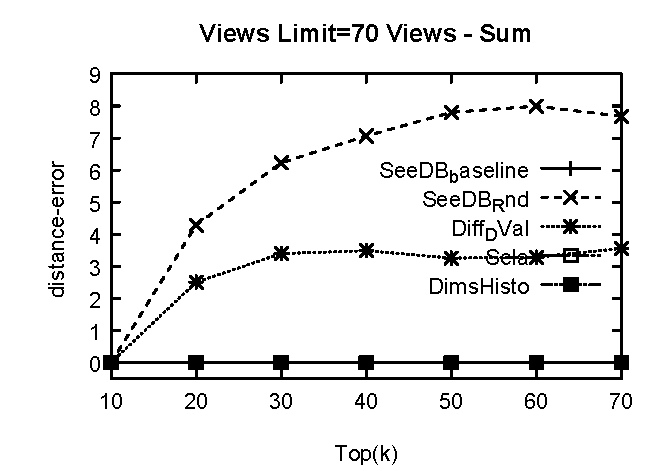
\includegraphics[width=\textwidth]{SumD1.pdf}
    \caption{Sum   }
        \label{fig:SumD1}%
  \end{subfigure}
  %
  \begin{subfigure}[b]{0.32\textwidth}
    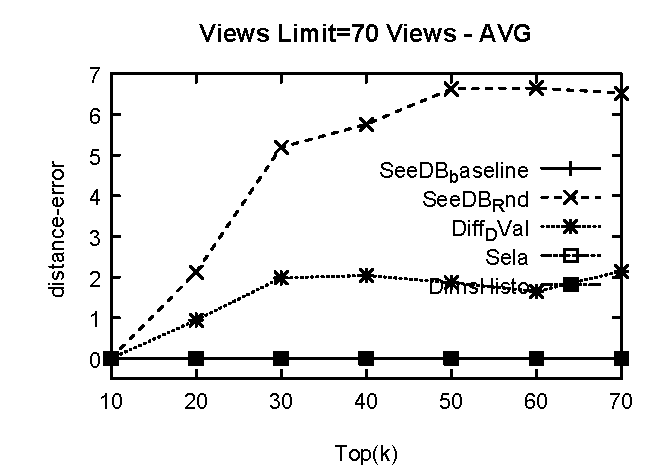
\includegraphics[width=\textwidth]{AvgD1.pdf}
     \caption{Average  }
        \label{fig:AvgD1}
  \end{subfigure}
  \begin{subfigure}[b]{0.32\textwidth}
    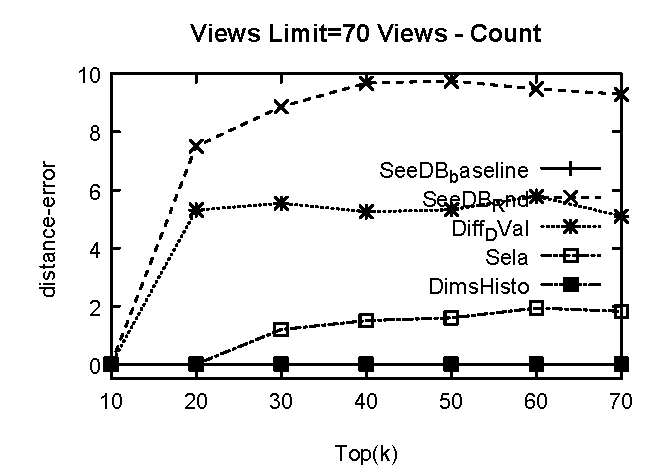
\includegraphics[width=\textwidth]{CountD1.pdf}
     \caption{count  }
        \label{fig:CountD1}
  \end{subfigure}
  \caption{Distance-error on varying k for the Algorithms $Sela$ ,$Diff_DVal$, $DimsHisto$, and $SeeDB_Rnd$}
\end{figure}


 % \begin{center}
    
  \begin{figure}[h]
  \centering
%\end{figure}
  \begin{subfigure}[b]{0.42\textwidth}
    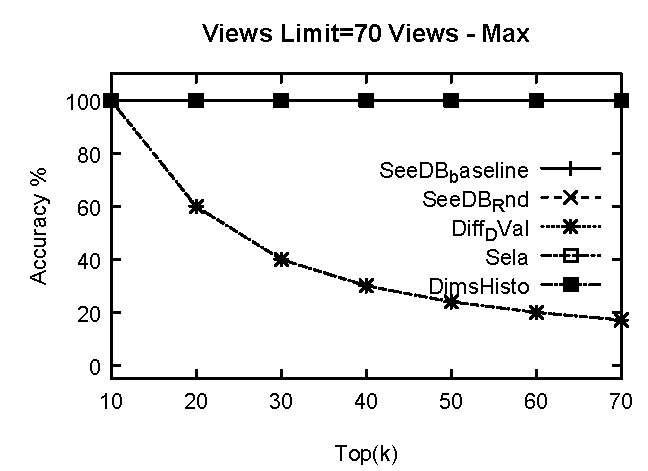
\includegraphics[width=\textwidth]{MaxA1.pdf}
    \caption{Max   }
        \label{fig:MaxA1}%
  \end{subfigure}
  %
  \begin{subfigure}[b]{0.42\textwidth}
    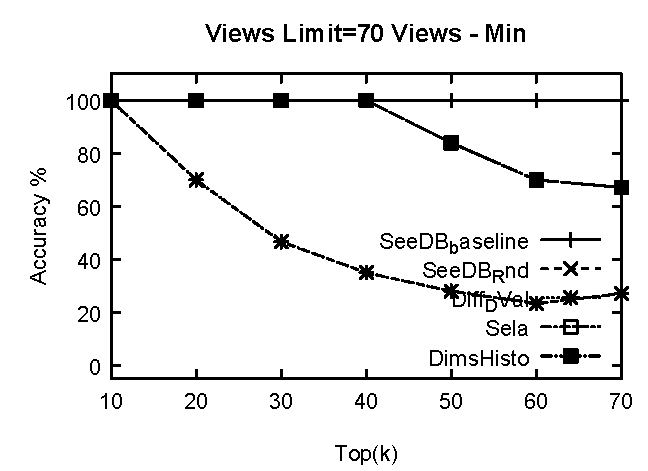
\includegraphics[width=\textwidth]{MinA1.pdf}
     \caption{Min  }
        \label{fig:MinA1}
  \end{subfigure}
  
  \caption{Accuracy on varying K for the Algorithms $Sela$ ,$Diff_DVal$, $DimsHisto$, and $SeeDB_Rnd$}
\end{figure}
%\end{center}

%\begin{center}
  
\begin{figure}[h]
  \centering
  \begin{subfigure}[b]{0.42\textwidth}
    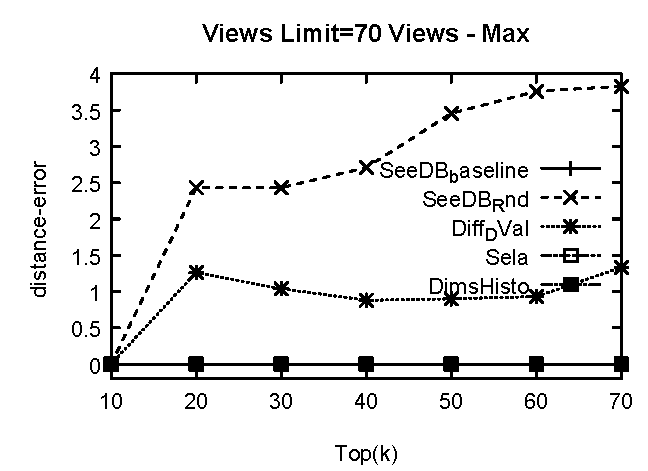
\includegraphics[width=\textwidth]{MaxD1.pdf}
    \caption{Max   }
        \label{fig:MaxD1}%
  \end{subfigure}
  %
  \begin{subfigure}[b]{0.42\textwidth}
    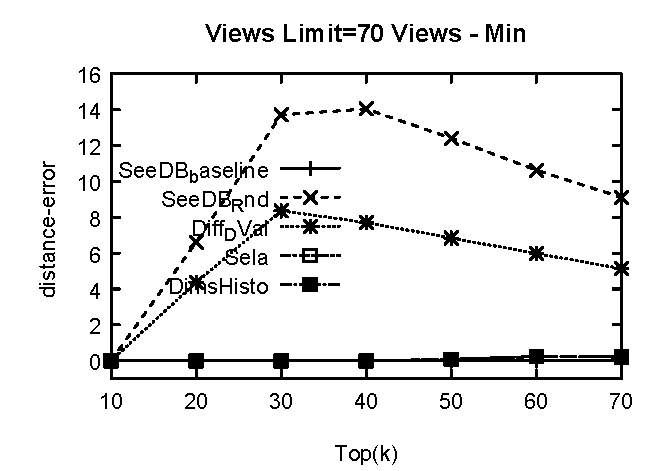
\includegraphics[width=\textwidth]{MinD1.pdf}
     \caption{Min  }
        \label{fig:MinD1}
  \end{subfigure}
  
  \caption{Distance-error on varying K for the Algorithms $Sela$ ,$Diff_DVal$, $DimsHisto$, and $SeeDB_Rnd$}
\end{figure}